\documentclass[letterpaper,12pt]{article}
\usepackage[utf8]{inputenc}

\usepackage{rotating}
\usepackage[top=1in, bottom=1in, left=1in, right=1in]{geometry}
\usepackage{graphicx}
\usepackage[numbers,square,sort&compress]{natbib}
\usepackage{setspace}
\usepackage[cdot,mediumqspace,]{SIunits}
\usepackage{hyperref}
\usepackage{mathtools}
\usepackage{url}
\usepackage{authblk}
\usepackage{placeins}
\usepackage{float}

\onehalfspacing
\title{Computational Physics Lab 11}
\author{Anita Bahmanyar}
\affil{\small {Student Number: 998909098}}
\date{November 28, 2014}

\usepackage{graphicx}

\renewcommand\thesubsection{\alph{subsection}}

\begin{document}

\maketitle

\section*{Q1}

%energy figure
\FloatBarrier
\begin{figure}[H]
\centering
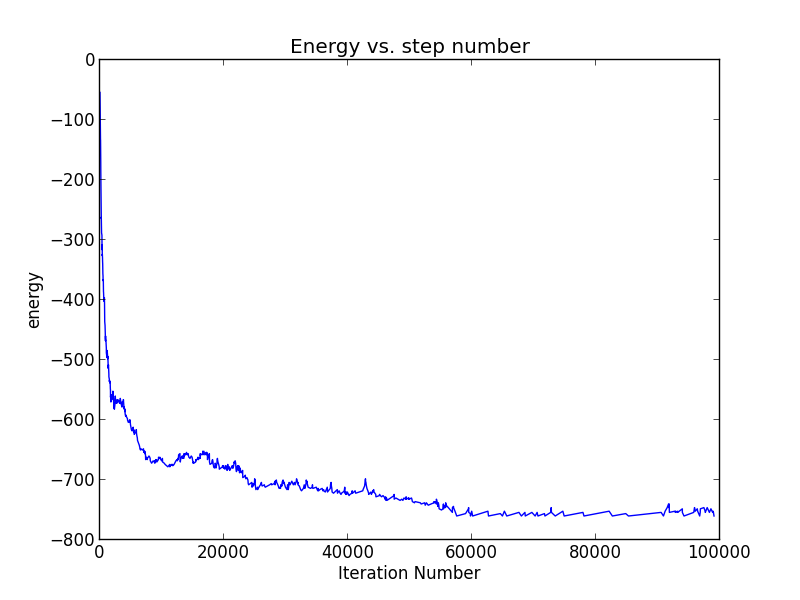
\includegraphics[scale=0.55]{q1_energy.png}
\caption{Energy of the spins vs. step number. As we increase the number of iteration, the energy goes to a lower value so that it minimizes the energy of the system.}
\end{figure}
\FloatBarrier

%magnetization figure
\FloatBarrier
\begin{figure}[H]
\centering
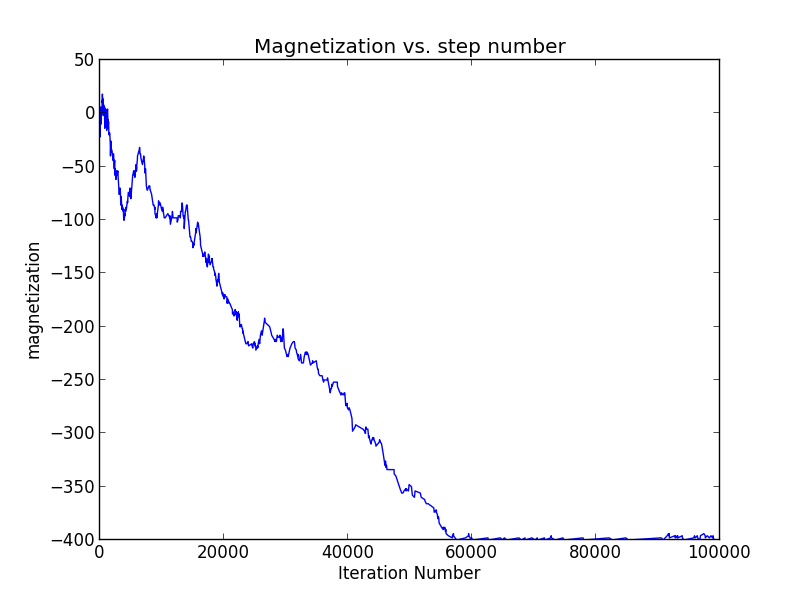
\includegraphics[scale=0.55]{q1_magnetization.png}
\caption{Magnetization of the spins. It starts with a number close to zero since there is a uniform probability for getting spin up and spin down, so the ration is almost the same. Then all the spins are magnetized either to spin 1 or spin -1.}
\end{figure}
\FloatBarrier

\section*{Q2}

% T = 1
\FloatBarrier
\begin{figure}[H]
\centering
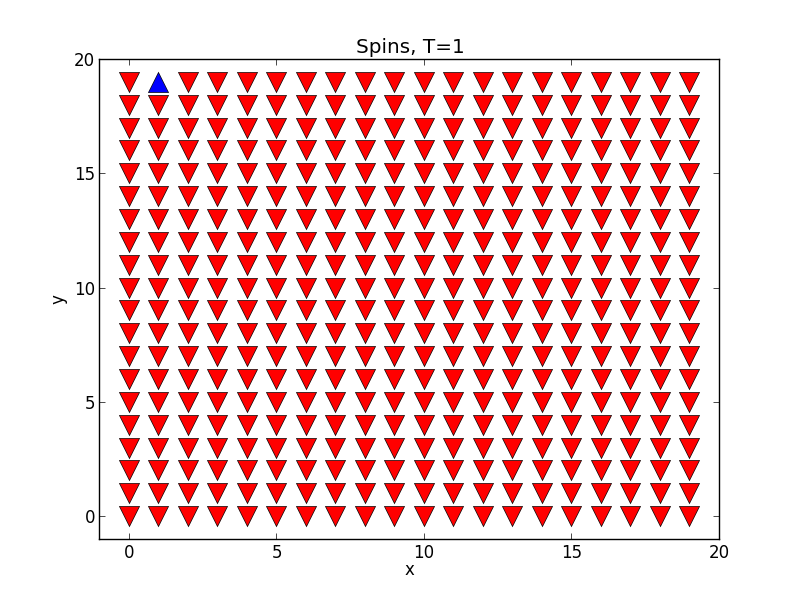
\includegraphics[scale=0.55]{q2_T1.png}
\caption{T=1.0}
\end{figure}
\FloatBarrier

% T = 1
\FloatBarrier
\begin{figure}[H]
\centering
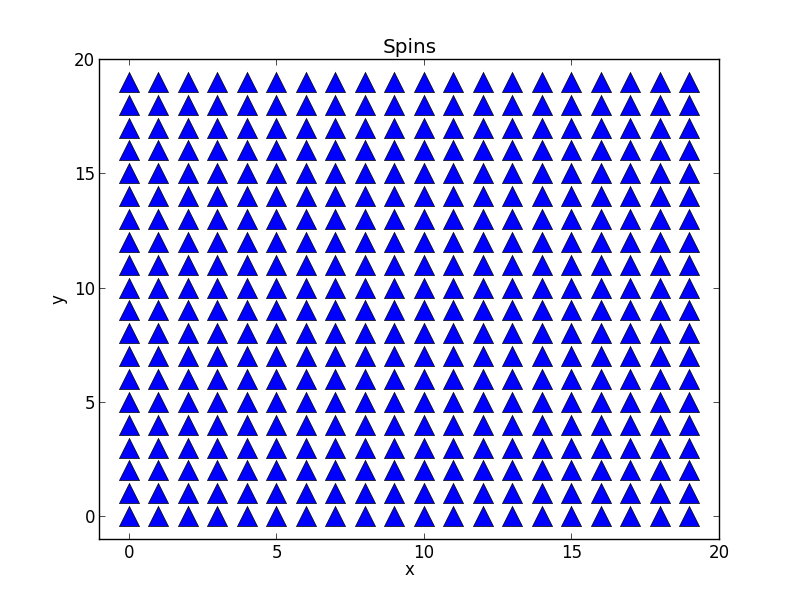
\includegraphics[scale=0.55]{q2_T11.png}
\caption{T=1.0}
\end{figure}
\FloatBarrier



% T = 2
\FloatBarrier
\begin{figure}[H]
\centering
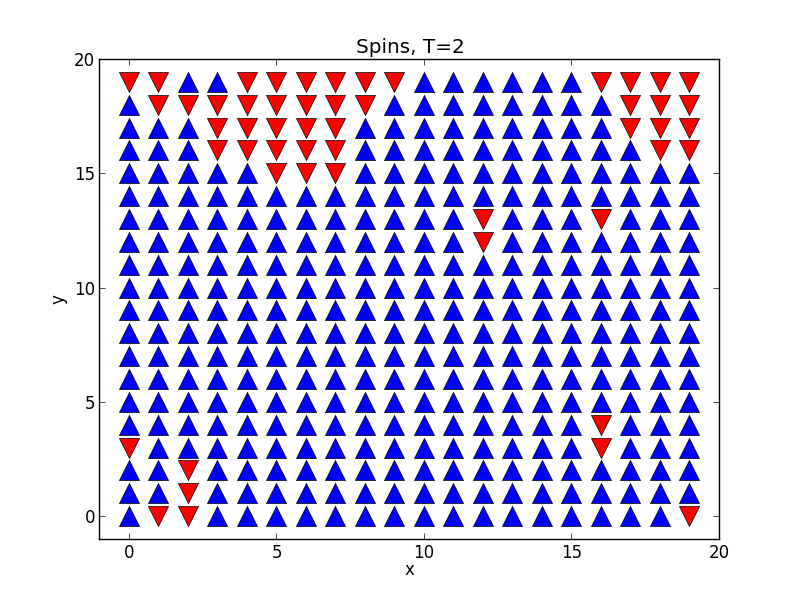
\includegraphics[scale=0.55]{q2_T2.png}
\caption{T=2.0}
\end{figure}
\FloatBarrier

% T = 3
\FloatBarrier
\begin{figure}[H]
\centering
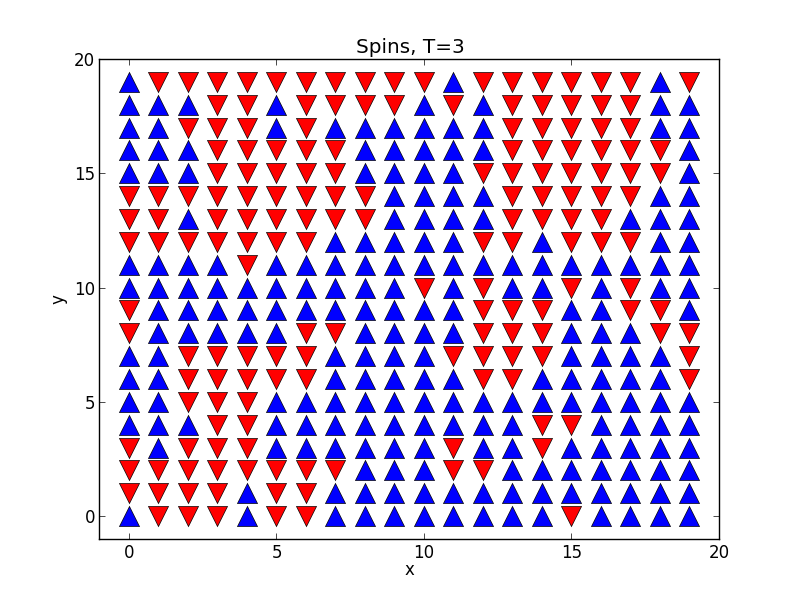
\includegraphics[scale=0.55]{q2_T3.png}
\caption{T=3.0}
\end{figure}
\FloatBarrier


As it is shown in the figures above, as the temperature is increased, there appears more difference in magnetization so there will be less uniform spin direction. In case of T=1 for instance, almost all of the spins are either up or down, whereas in cases T=2 and T=3, there is a combination of both and gets to a combination of the two more with increasing temperature.

\section*{Q3}

%
\FloatBarrier
\begin{figure}[H]
\centering
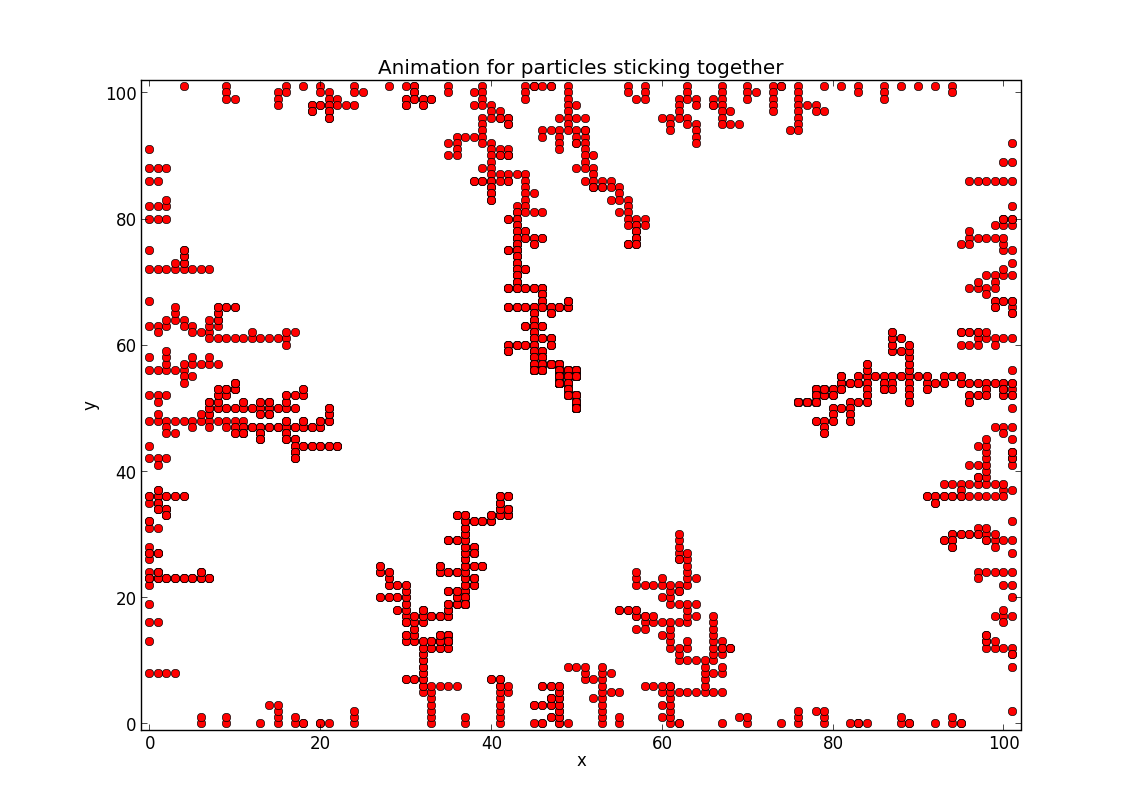
\includegraphics[scale=0.55]{q3.png}
\caption{}
\end{figure}
\FloatBarrier

\end{document}


